%-------------------------------------------------------------------------------
%                                PREAMBLE
%-------------------------------------------------------------------------------
\documentclass[usenames,dvipsnames,svgnames,9pt]{beamer}
\usetheme{flow} % This theme uses TIKZ: compile twice with PDFLaTeX or LuaLaTeX.
%\cleanslidestrue

\usepackage{hyperref,graphicx,lmodern}
\usepackage[utf8]{inputenc}

\graphicspath{{imgs/}}


%-------------------------------------------------------------------------------
%                                TITLE PAGE
%-------------------------------------------------------------------------------
\title[footline~title] % Short title used in footline
{
	A long title as a test % Long title
}

\author[P.~Author:] % Presenting author in short form used in footline
{
	\underline{First Author}$^1$, Second Author$^2$ and Third Author$^1$
}
% - Give the names in the same order as the appear in the paper.
% - Underline the presenting author.

\institute[unused]
{
	$^1$Linn\'e FLOW Centre, KTH Mechanics\\
	$^2$DAST, Politecnico di Milano
}
% Keep it simple, no one is interested in your street address.

% University logo(s)
\logot{
\includegraphics[width=.105\paperwidth]{KTH-logo}}  % Top logo
\logob{
\includegraphics[width=.105\paperwidth]{Flow-logo}} % Bottom logo
\logoc{
\includegraphics[width=.105\paperwidth]{PoliMi-logo}} % Corner logo
%
% Cover image: \cvrimg{x position}{y position}{cover image}
\cvrimg{.77}{.75}{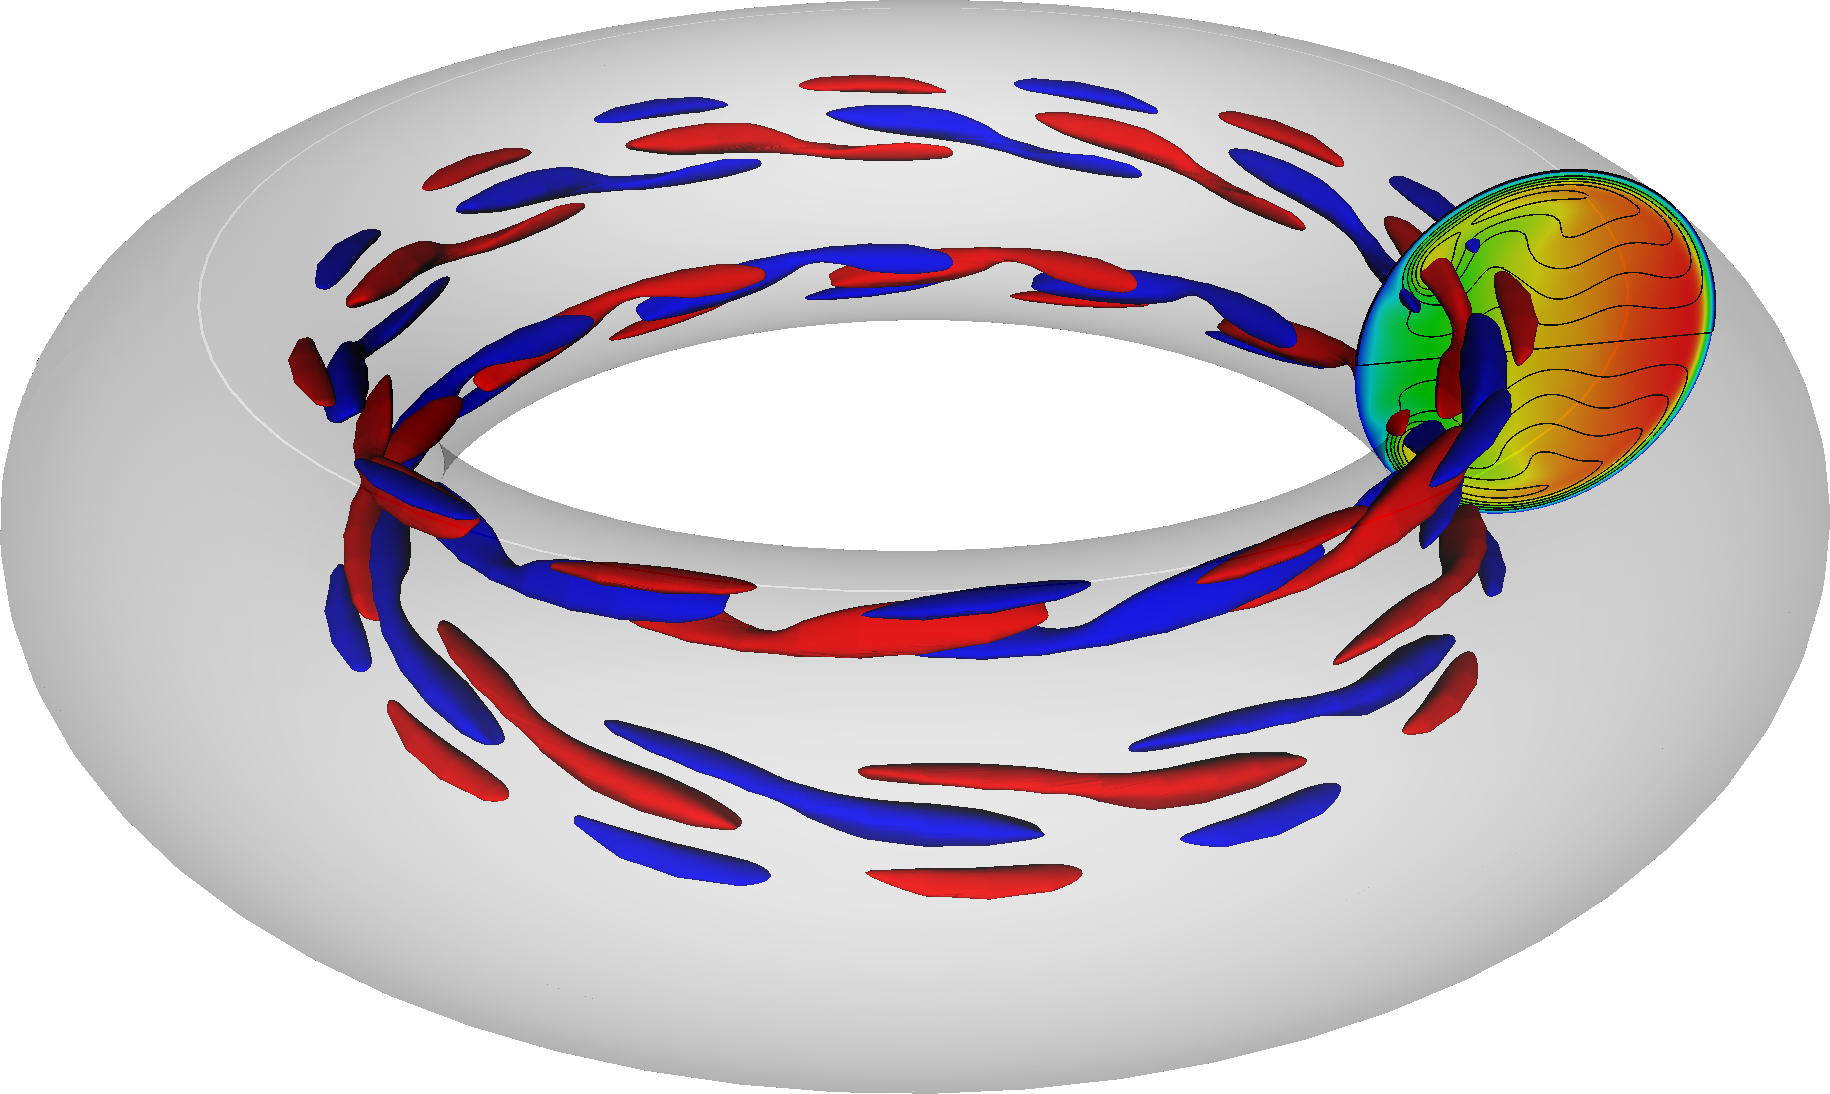
\includegraphics[width=.4\paperwidth]{cover-image}}

\date[unused]
	{Conference name -- date}
% - Either use conference name or its abbreviation.
% - Not really informative to the audience, more for people (including
%   yourself) who are reading the slides online

% Uncomment this if you want the table of contents to pop up at the 
% beginning of each section (you can do the same with subsections):
%\AtBeginSection[]
%{
%  \begin{frame}<beamer>
%    \tableofcontents[currentsection,currentsubsection]
%  \end{frame} \addtocounter{framenumber}{-1}
%}

% If you wish to uncover everything in a step-wise fashion, uncomment
% the following command: 
% \beamerdefaultoverlayspecification{<+->}


\begin{document}

\titleframe % Print the title as the first slide


%-------------------------------------------------------------------------------
%                           PRESENTATION SLIDES
%-------------------------------------------------------------------------------

\section{Section title}

\begin{frame}[t]{Slide title}
	{and subtitle}
  
  Something to show the textwidth of this Linn\'e FLOW Centre beamer template.
  
  \begin{itemize}
    \item This is an item.
    \item This is also an item.
    \item ...
  \end{itemize}
    
\end{frame}

\begin{frame}[t]{Frame coordinate system}
	{absolute positioning of images and sketches}
	%
	% Coordinate system for the page:
	%
	% -------------------------
	% |(0,1)             (1,1)|
	% |                       |
	% |       (0.5,0.5)       |
	% |                       |
	% |(0,0)             (1,0)|
	% -------------------------
	%
	% invoke by:
	% \node[nodeOptions] (nodeName) at (page cs:xNode,yNode) {nodeContents};

	\begin{tikzpicture}[remember picture,overlay]
		\node (sw) at (page cs:0,0) {+}; % bottom left
		\node (se) at (page cs:1,0) {+}; % bottom right
		\node (ne) at (page cs:1,1) {+}; % top    right
		\node (nw) at (page cs:0,1) {+}; % top    left

		\draw (sw) -- (se) -- (ne) -- (nw) -- cycle; % outer rectangle
		\draw (sw) -- (ne); % diagonals
		\draw (se) -- (nw); % diagonals

		\node (ce) at (page cs:0.5,0.5) {+}; % center

		\node (image) at (page cs:0.75,0.75) {% 
			
\includegraphics[width=.105\paperwidth]{Flow-logo}%
		};
	\end{tikzpicture}
    
\end{frame}

%-------------------------------------------------------------------------------


\thanksframe \label{final-frame}

\end{document}
